\documentclass[a4paper,11pt]{report}
\usepackage[utf8]{inputenc}
\usepackage{graphicx}
\usepackage{url}
\usepackage{cite}
\usepackage{multicol}


\setlength{\topmargin}{-0.25in}
\setlength{\headheight}{0in}
\setlength{\textheight}{9.5in}
\setlength{\headsep}{0in}
\setlength{\oddsidemargin}{-0.25in}
\setlength{\evensidemargin}{-0.25in}
\setlength{\textwidth}{7.0in}


%opening
\title{{\bf Assignment-4 CS401} }
%\numberofauthors{2}
\author{Abhishek Pratap singh\\
kush@cse.iitb.ac.in}

\begin{document}
\maketitle
\tableofcontents
 \section{Scheduler level statistics}
 \subsection{Experiment 1: Load vs Context Switches}
  In this experiment on x axis no of cpu intensive process currently running on system (0..11...88)\\ .
  and reading for context switches taken for 10 seconds each time.\\
  experiment done upto maximum load handling power of system.\\
  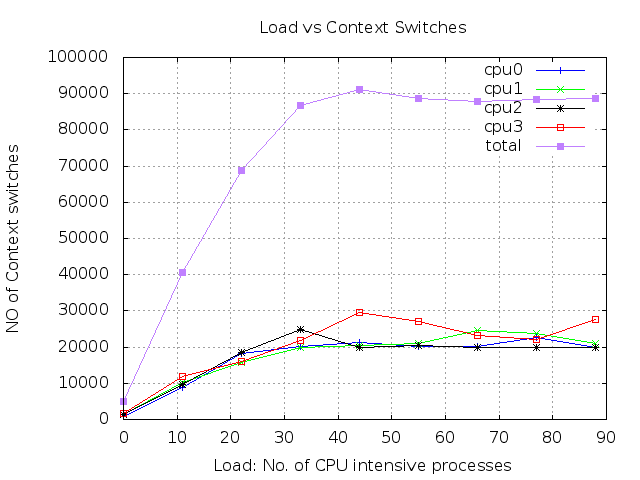
\includegraphics[scale=0.6]{loadvscs.png}
  \\{\bf conclusion:} No of context increases with load but for a particular cpu it decrease some time due load balancing among CPUs.\\
   total context switches increases with load then after some time it becomes statistically constant due to limitation of load handling capability of system and hardware.
 \subsection{Experiment 2: Run Queue length distribution per CPU}
 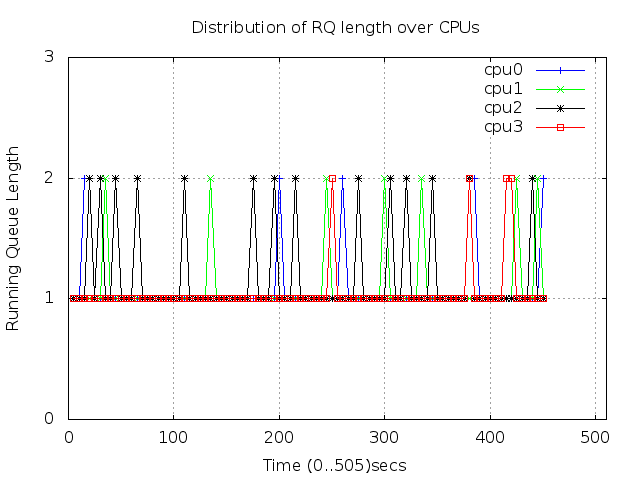
\includegraphics[scale=0.6]{rqlength.png}
 \subsection{Experiment 3: Number of Migrations across CPUs}
 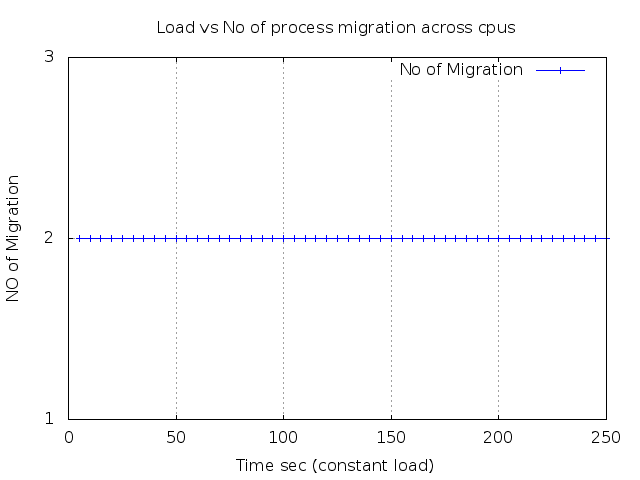
\includegraphics[scale=0.6]{mig1.png}\\
 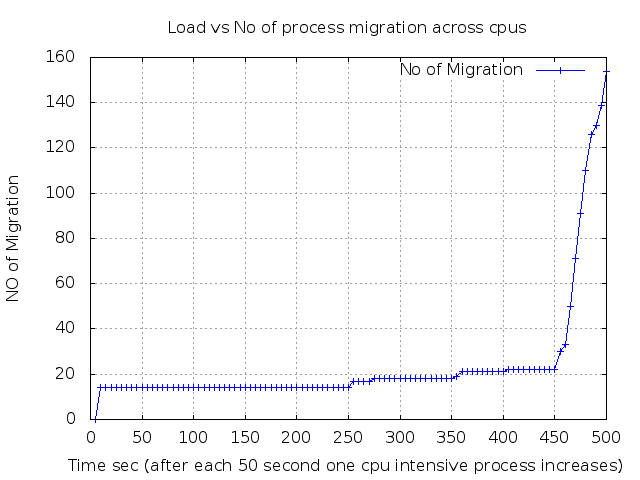
\includegraphics[scale=0.6]{mig2.png}
 \subsection{Experiment with scheduling priorities}
 There are two cpu intensive process \\
 one with 20 nice value \\
 and other is -20 value
 \subsection{context switches vs time}
 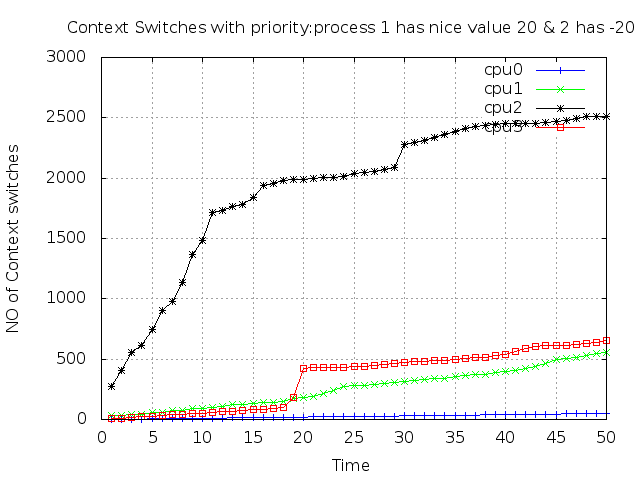
\includegraphics[scale=0.6]{priosched.png}
 \subsection{No. of migration}
  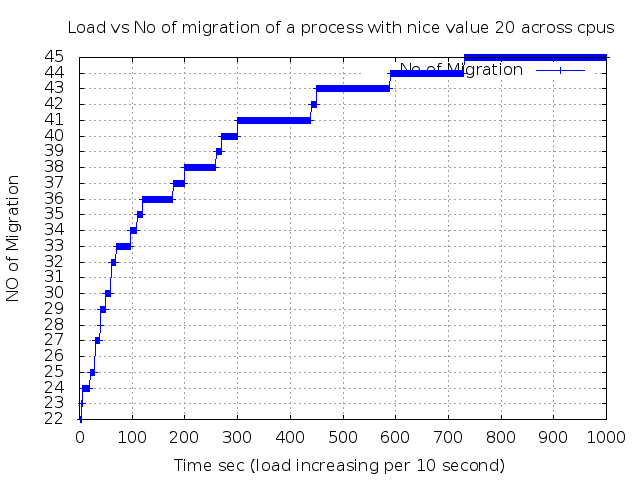
\includegraphics[scale=0.6]{miglow.png}
 \section{Process level Statistics}
 \subsection{Number of context switches}
 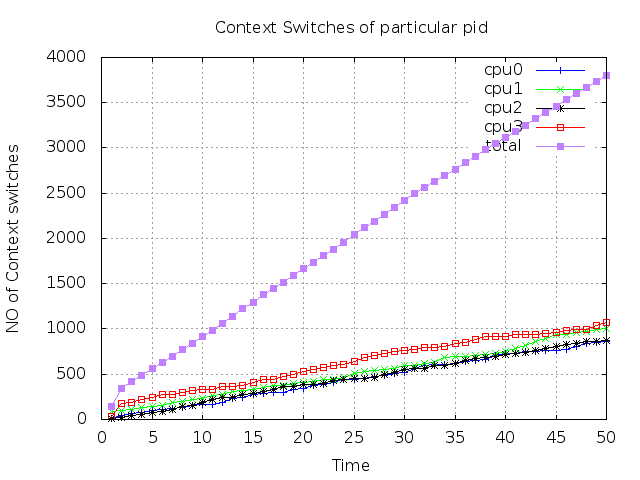
\includegraphics[scale=0.6]{pidcs.png}
 
 \subsection{Variation in dynamic priority of the process}
 \subsection{CPU mapping distribution of process}
 \subsection{Experiments with CPU affinity of process}



\end{document}
